\documentclass[aps, pre, onecolumn, nofootinbib, notitlepage, groupedaddress, amsfonts, amssymb, amsmath, longbibliography, superscriptaddress]{revtex4-1}
\usepackage{tabularx}
\usepackage{graphicx}
\usepackage{hyperref}
\usepackage{xcolor}
\hypersetup{
    colorlinks,
    linkcolor={red!50!black},
    citecolor={blue!50!black},
    urlcolor={blue!80!black}
}
\usepackage{bm}
\usepackage{natbib}
\usepackage{longtable}
\LTcapwidth=0.87\textwidth

\newcommand{\Div}[1]{\ensuremath{\nabla\cdot\left( #1\right)}}
\newcommand{\DivU}{\ensuremath{\nabla\cdot\bm{u}}}
\newcommand{\angles}[1]{\ensuremath{\left\langle #1 \right\rangle}}
\newcommand{\KS}[1]{\ensuremath{D_{\text{KS}}(#1)}}
\newcommand{\KSstat}[1]{\ensuremath{\overline{D_\text{KS}(#1)}}}
\newcommand{\grad}{\ensuremath{\nabla}}
\newcommand{\RB}{Rayleigh-B\'{e}nard }
\newcommand{\Reff}{\ensuremath{\text{Re}_{\text{ff}}}}
\newcommand{\Peff}{\ensuremath{\text{Pe}_{\text{ff}}}}
\newcommand{\stressT}{\ensuremath{\bm{\bar{\bar{\Pi}}}}}
\newcommand{\lilstressT}{\ensuremath{\bm{\bar{\bar{\sigma}}}}}


\newcommand\mnras{{MNRAS}}%
\newcommand\apjl{{The Astrophysical Journal Letters}}%

\begin{document}
%\author{Evan H. Anders}
%\affiliation{Dept. Astrophysical \& Planetary Sciences, University of Colorado -- Boulder, Boulder, CO 80309, USA}
%\affiliation{Laboratory for Atmospheric and Space Physics, Boulder, CO 80303, USA}

\title{Additions to ch2 postscript / ch7.5 revamp}

\maketitle

%%%%%%%%%%%%
%%%%%%%%%%%
% INTRO
%%%%%%%%%%%
%%%%%%%%%%%%

\section{Addition to Ch2 Postscript: Control Parameters Examination}
The fully compressible equations, as presented in 2.4-2.6, are in their nondimensionalized form in which we solved the equations.
Thermodynamics are nondimensionalized to unity at the top of the atmosphere, length scales are nondimensionalized to temperature gradient length scale at the top of the domain, and timescales are nondimensionalized to the sound-crossing time of that unit length.
In these equations, the diffusivities are straightforwardly set by the input values of Ra$_t$ and Pr, and do not evolve over time.
In addition to the diffusivities, the other remaining control parameter is $\epsilon$ or $\Delta s$, the magnitude of the entropy fluctuations (and thus the magnitude of thermodynamic fluctuations), which \emph{may} evolve over time.
In addition to these three control parameters, convection occurs in an atmosphere, the stratification of which will evolve over time, and will differ from the initial state by O($\epsilon$).

$\Delta s$ appears in the definition of Ra, so if it evolves appreciably, then it's possible that the input value of both Ra and $\epsilon$ are different from the values achieved in the evolved system.
If we had chosen fixed-entropy boundary conditions, we would know that $\epsilon$ would remain constant.
However, it is unclear how $\epsilon$ changes under our choice of fixed-\emph{temperature} boundary conditions.
So -- Let's examine how $\Delta s$ evolves further.

For an alternative nondimensionalization of the equations which is perhaps more straightforward, I refer the reader to section \ref{sec:freefall_nondim} where the equations are nondimensionalized on a freefall timescale and cast in terms of more traditional nondimensional terms.

\subsection{The magnitude of $\Delta s$}
In order to find the imposed entropy jump across our convective domain, we start with the entropy equation,
\begin{equation}
\frac{1}{c_P}\grad s = \frac{1}{\gamma}\grad\ln T - \frac{\gamma - 1}{\gamma}\grad \ln \rho,
\end{equation}
where $s$ is the specific entropy, $T$ is the temperature, $\rho$ is the density, $\gamma$ is the adiabatic index, and $c_P$ is the specific heat at constant pressure.
After horizontally averaging this equation and integrating it from the bottom to the top of our domain, we find
$$
\frac{\Delta s}{c_P} = \int_0^{L_z} \frac{\partial s}{\partial z} dz = \frac{1}{\gamma}\left(\ln T\bigg|_{z=0}^{z=L_z} - (\gamma-1)\ln\rho\bigg|_{z=0}^{z=L_z}\right).
$$
Under our choice of fixed-temperature boundary conditions, $T(z=0) = T_b$ and $T(z=L_z) = T_t$, both of which are constants.
Furthermore, we note that $\ln(\rho_t/\rho_b) = -n_\rho$, the number of density scale heights, which can evolve.
So the entropy jump across our domain is
\begin{equation}
\frac{\Delta s}{c_P} = \frac{1}{\gamma}\ln\left(\frac{T_t}{T_b}\right) + \frac{\gamma-1}{\gamma} n_\rho(t).
\end{equation}
For our nondimensional polytropes, $T_t = 1$ and $T_b = 1 + L_z$, where we define $L_z = e^{n_\rho/m} - 1$.
This means $\ln (T_t/T_b) = \ln (e^{-n_{\rho,0}/m}) = -n_{\rho,0}/m$, where $n_{\rho,0}$ is the value of $n_\rho$ in the initial atmosphere and $m$ is the polytropic index.
Decomposing $n_\rho(t) = n_{\rho,0} + \Delta n_\rho(t)$, we find
\begin{equation}
\frac{\Delta s}{c_P} = \frac{1}{\gamma}\left((\gamma-1)n_{\rho,0} - \frac{n_{\rho,0}}{m}\right) + \frac{\gamma-1}{\gamma}\Delta n_\rho(t).
\end{equation}
Also recall that $m = m_{\text{ad}} - \epsilon$ and $m_{\text{ad}} = (\gamma-1)^{-1}$, such that we can simplify this expression to 
\begin{equation}
\frac{\Delta s}{c_P} = \frac{\gamma-1}{\gamma}\left( -\epsilon \frac{n_{\rho,0}}{m} + \Delta n_\rho(t)\right).
\label{eqn:deltaS_evolved}
\end{equation}
In other words, this is some O($\epsilon$) quantity that evolves with the number of density scale heights of the evolved atmosphere.
So -- let's try to put some boundaries on the value of $\Delta n_\rho(t)$.

\subsection{Estimates for changes in $n_\rho$}
We can't know this a priori -- if we did, we wouldn't need to run the convection simulation because we'd know the boundary layer structure (and thus stuff like the Nusselt number) in advance.
But -- we can build a simple model to get a feel for how $n_\rho$ will evolve.
We know that the atmospheric density stratification will evolve under two constraints:
\begin{enumerate}
\item Mass is conserved, and
\item Adiabaticity is achieved throughout most of the domain (the convective interior, not the boundary layers).
\end{enumerate}
Our choice of fixing the temperature at the top and bottom boundaries means that the adiabat that our simulation ``chooses'' in the convective interior will be bounded by two adiabats that we know about: the adiabat that crosses the top boundary temperature ($T = 1$ at $z = L_z$) and the adiabat that crosses the bottom boundary temperature ($T = 1 + L_z$ at $z = 0$).
We further know the adiabatic temperature gradient for our nondimensionalization, $\grad_{\text{ad}} = -g / c_P \hat{z} = (-1 + \epsilon/c_P)\hat{z}$.
I will therefore set up two types of model temperature profiles to understand the density behavior of boundary layers:
\begin{equation}
\partial_z T_{\text{top-BL}} = \begin{cases}
\grad_{\text{ad}} & z < (1-\delta) L_z, \\
\grad_{\text{s}}  & z \geq (1-\delta) L_z, \,\, |\grad_{\text{s}}| > |\grad_{\text{ad}}|
\end{cases},\qquad
\partial_z T_{\text{bot-BL}} = \begin{cases}
\grad_{\text{ad}} & z > \delta L_z, \\
\grad_{\text{s}}  & z \leq \delta L_z, \,\, |\grad_{\text{s}}| > |\grad_{\text{ad}}|
\end{cases}.
\end{equation}
Here, $T_{\text{top-BL}}$ is an atmosphere that is adiabatic everywhere except for a superadiabatic boundary layer of width $\delta L_z$ at the top of the domain.
Similarly, $T_{\text{bot-BL}}$ is adiabatic everywhere except for a superadiabatic boundary layer at the bottom of the domain (of width $\delta L_z$).
In these models, $\delta < 1$ is the fraction of the domain that the boundary layer occupies.
The value of the superadiabatic temperature gradient is $\grad_{\text{s}} = [(T_t - T_b) - \grad_{\text{ad}} L_z (1 - \delta)] / (\delta L_z)$, and is determined by our choice of fixed-temperature boundary conditions.
For a given value of $\epsilon$ and $\delta$, the temperature solution is precisely defined.

\begin{figure}[t!]
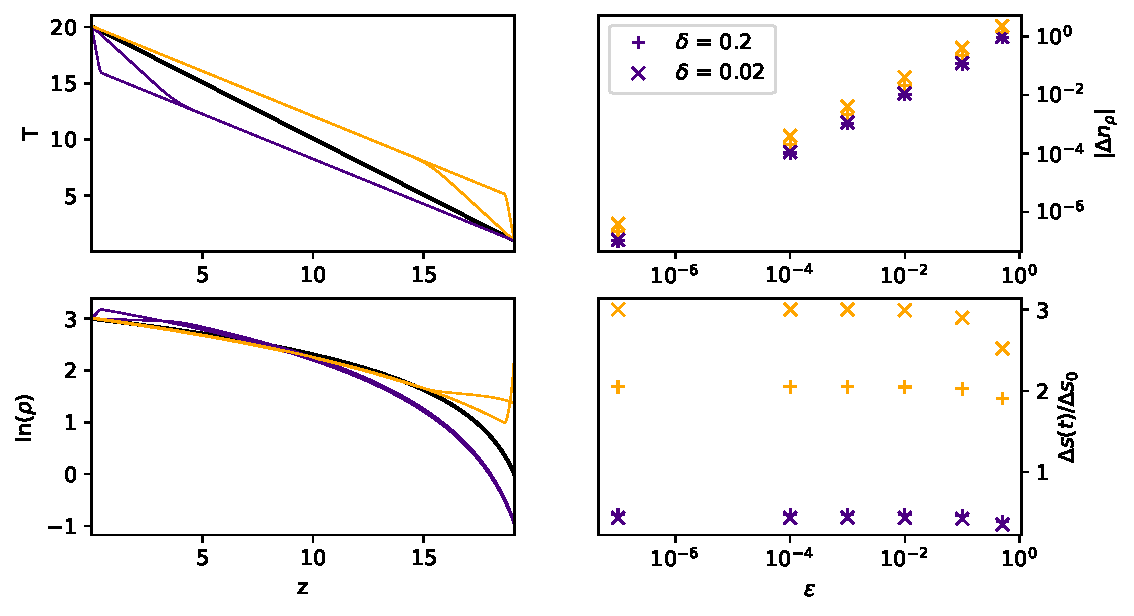
\includegraphics[width=\textwidth]{./atmospheres/limiting_adiabats.pdf}
\caption{ (left two panels) Stratification of simple atmospheric solutions with upper and lower boundary layers are shown.
		  Temperature (upper left) and log density (lower left) are shown, and the initial state (an $\epsilon = 0.5$ polytrope) is shown in black.
		  Orange profiles show atmospheres which are perfectly adiabatic everywhere except for an upper boundary layer, and purple profiles show profiles which are adiabatic other than a lower boundary layer.
		  All shown atmospheres have the same $\Delta T$ across the domain and the same mass.
		  (upper right) Changes in $n_\rho$ from profiles similar to those in the left panels at many different values of $\epsilon$.
		  Purple points correspond to lower boundary layers and are positive; orange points correspond to upper boundary layers and are negative.
		  The shape of the marker shows the difference between a thicker boundary layer (0.2 or 20\% of the domain) vs.~ a thinner boundary layer (0.02 or 2\%).
		  $\Delta n_\rho$ scales with $\epsilon$, as expected.
		  In the lower right panel, we calculate the evolved $\Delta s$ according to Eqn.~\ref{eqn:deltaS_evolved} and normalize it by the initial $\Delta s$.
		  We find that upper boundary layers make the atmosphere more superadiabatic and lower boundary layers make the atmosphere more adiabatic.
	\label{fig:limiting_adiabats} }
\end{figure}




To understand how these boundary layers respectively affect the density stratification, and therefore the entropy jump across the domain, we can solve a simple mass-conserving boundary value problem for hydrostatic equilibrium, 
\begin{equation}
\begin{split}
\frac{\partial M}{\partial z} = \rho,\\
T\frac{\partial \ln\rho}{\partial z} + \frac{\partial T}{\partial z} = -g,
\end{split}
\end{equation}
under the constraints that $M = 0$ at $z = 0$ and $M = \int_0^{L_z} \rho_0 dz$ at $z = L_z$, where $\rho_0$ is the initial density stratification of the polytrope.
In the left two panels of Fig.~\ref{fig:limiting_adiabats}, some examples of these temperature and density profiles can be seen.
The cases shown have $\epsilon = 0.5$, to ensure that the changes away from the initial state are appreciable and observable.
The orange lines show profiles of $T_{\text{top-BL}}$ and the purples lines show profiles of $T_{\text{bot-BL}}$; for both cases, we solve for $\delta = \{0.2, 0.02\}$.
The changes in $\ln\rho$ are qualitatively similar to the changes observed in Fig.~2.4, and we generally find that: bottom boundary layers aim to \emph{increase} $n_\rho$ while upper boundary layers aim to \emph{decrease} $n_\rho$.
This means that bottom boundary layers try to stabilize the system (through atmospheric slumping) and top boundary layers further destabilize the system (through density inversions).

We performed this analysis for a broad range of $\epsilon = [10^{-7}, 0.5]$, and we show the magnitude of $\Delta n_\rho$ as a function of $\epsilon$ in the upper right panel.
In all cases, $\Delta n_\rho$ for the orange (upper boundary layer) points are negative while the purple (lower boundary layer) points are positive.
In the lower right panel, we solve Eqn.~\ref{eqn:deltaS_evolved} for $\Delta s$, and normalize it by its input value.
We find that upper boundary layers aim to increase the magnitude of $\Delta s$, effectively increasing the input value of $\epsilon$ (by a factor of $\sim 2-3$).
Lower boundary layers, on the other hand, aim to decrease the magnitude of $\Delta s$, effectively decreasing the input value of $\epsilon$ (by a factor of, again, $\sim 2-3$).
In our published work (Fig.~2.4), we find that the upper boundary layer effects tend to dominate, so it's reasonable to assume that $\Delta s$ will increase in magnitude by a factor of a few away from the initial conditions.

\subsection{Experimentally measured changes in $n_\rho$}
Fortunately, when I did this work in 2017, I included the evolved value of $n_\rho$ in a supplementary \texttt{.csv} file.
Unfortunately, when I did this work, I was fairly new to computing, and I made a bit of a rookie mistake: I output the volume-integrated value of the \emph{full} $n_\rho$, not $\Delta n_\rho$.
The output operations that I used are less accurate than our simulations, so very small O($\epsilon$) changes on the initial value of $n_\rho = 3$ were not successfully preserved in the data.
For our $\epsilon = 10^{-4}$ cases, this means that the values of $n_\rho$ I am presenting here are, to first order, accurate -- but noisier than they should be.
Unfortunately, the signal of evolved flows for $\epsilon = 10^{-7}$ was lost, so I am not including those points in this analysis.

Using Eqn.~\ref{eqn:deltaS_evolved}, I calculated the evolved $\Delta s$ in my simulations and normalized it by the input value.
I've plotted this in the left panel of Fig.~\ref{fig:delta_S_vs_ra}.
We can see that the magnitude of $\Delta s$ increases by a factor of a few over many decades of Ra in both 2D and 3D.
If we calculate the value of Ra in the evolved state through the formula,
$$
\text{Ra}_{t, \text{evolved}} = \frac{\Delta s_{\text{evolved}}}{\Delta s_{\text{initial}}} \text{Ra}_{t},
$$
and plot $\text{Ra}_{t, \text{evolved}}$ vs.~$\text{Ra}_{t}$ in the right panel of Fig.~\ref{fig:delta_S_vs_ra}, we see that while we don't perfectly achieve a 1-to-1 input-to-output ratio, we achieve something close to that.
Furthermore, for the larger values of $\epsilon$ where I trust this measurement more, it seems like the evolved $\Delta s$ plateaus around Ra $\sim 10^4$ (similar to where those cases become supersonic), so $\epsilon$ and Ra are truly independent input parameters for our most turbulent 2D simulations.

\textbf{In summary, while $\epsilon$ and Ra are not \emph{perfectly} independent control parameters for our fixed-temperature boundary conditions, they are nearly independent.
The evolution of the density profile does not change the entropy jump by more than a factor of a few from the initial state.}


\begin{figure}[t!]
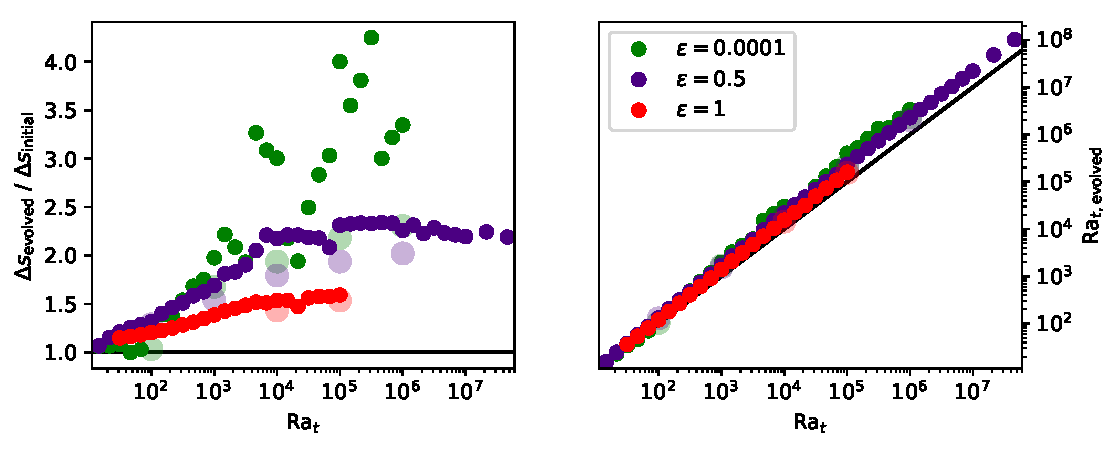
\includegraphics[width=\textwidth]{./figs/delta_S_vs_ra.pdf}
\caption{ (left) Measured values of $\Delta s$, from Eqn.~\ref{eqn:deltaS_evolved}, using values of $\Delta n_\rho$ obtained from our simulations.
		  2D points are small, dark circles while 3D points are large, light-colored circles.
		  (right) The corresponding changes in Ra resulting from the small observed changes in $\Delta s$.
		  The ideal 1-to-1 correspondence between input and output Ra is plotted as a black line, and it is close to the achieved scaling.
	\label{fig:delta_S_vs_ra} }
\end{figure}


\subsection{Mach number evolution in 2D vs.~3D}
The difference in the behavior of Ma vs.~Ra in 2D and 3D (shown in Fig.~2.1) remains a bit of a mystery.
If the scaling of Mach number with Ra in 2D were a result of $\Delta s$ increasing in magnitude, the data in Fig.~\ref{fig:delta_S_vs_ra} would suggest that Mach number should similarly grow with increasing Ra in 3D.
We find (Fig.~\ref{fig:delta_S_vs_ra}) that the magnitude of $\Delta s$ grows with Ra in both 2D and 3D, and the Mach number should also therefore grow.
However, $\Delta s$ changes only by a factor of 2-4, at most, from onset through the most turbulent simulations that we studied.
We would therefore expect Mach to change by $\sqrt{2-4}$, at most, as a result of $\Delta s$ changes.
This is not what we observe; in 3D, the Mach number at fixed $\epsilon$ is constant as a function of increasing Ra, while the Mach number in 2D increases by more than an order of magnitude across the range of Ra we studied.
This disagreement suggests that changes to the entropy stratification are not the primary cause of the scaling of Ma with Ra in 2D.

The scaling of Ma vs.~Ra in 2D is an open question and figuring out what causes it is beyond the scope of this thesis.
A careful examination of this phenomenon and an understanding of the mechanisms behind it are enough work to justify a full paper.
Regardless, what we know about this scaling is as follows:
\begin{enumerate}
\item Velocities grow with increasing Ra in 2D but not 3D in our experimental setup.
\item Morphologies are very different in 2D and 3D (2D exhibits a large, coherent ``flywheel,'' 3D does not.)
\item At low Mach number, eventually 2D cases break apart these flywheels and exhibit ``shearing'' states, much like in Boussinesq convection.
\item The scaling of Ma vs.~Ra stops when Ma = 1.
\end{enumerate}
Phenomenologically, low-Ma 2D compressible convection behaves very similarly to Boussinesq convection.
To my knowledge, no one has carefully studied why high-velocity flywheel modes are so favored by 2D convection; it's possible that these modes are a result of inverse turbulent cascades in 2D, but that's pure speculation.
This work here does not explain our observed Ma~vs.~Ra scaling, but it does rule out the hypothesis that it is caused by entropy restratification.

\newpage




\section{A Revamped section 7.5: A clearer freefall nondimensionalization of the equations}
\label{sec:freefall_nondim}
The (dimensional) form of the fully compressible equations solved in ch.~2 is 
\begin{align}
&\begin{aligned}
&\frac{\partial \ln\rho}{\partial t} + \grad\cdot\bm{u} 
    = -\bm{u}\cdot\grad\ln\rho,
	\label{eqn:ab17continuity_eqn}
\end{aligned}\\
&\begin{aligned}
\frac{\partial\bm{u}}{\partial t} + R \grad T - 
&\nu\grad\cdot\lilstressT - \lilstressT\cdot\grad\nu =
-\bm{u}\cdot\grad\bm{u} - RT\grad\ln\rho + \bm{g} + 
\nu\lilstressT\cdot\grad\ln\rho,
\label{eqn:ab17momentum_eqn}
\end{aligned}\\
&\begin{aligned}
\frac{\partial T}{\partial t} -\frac{1}{c_V}\left(\right.\chi&\left.
    \grad^2 T + \grad T\cdot\grad\chi\right) =
	-\bm{u}\cdot\grad T - (\gamma-1)T\grad\cdot{\bm{u}}
	+ \frac{1}{c_V}\left(\chi\grad T \cdot\grad\ln\rho +
	\nu\left[\lilstressT\cdot\nabla\right]\cdot\bm{u}\right), 
	\label{eqn:ab17energy_eqn}
\end{aligned}
\end{align}
Here, $\bm{u}$ is the velocity, $\rho$ is the density, $T$ is the temperature, $R$ is the ideal gas constant (where the pressure $P = R\rho T$), $\bm{g}$ is the gravitational acceleration, $\lilstressT$ is the viscous stress tensor (in units of inverse time), $c_V$ is the specific heat at constant volume, and $\nu$ and $\chi$ are respectively the viscous and thermal diffusivities (in units of length$^2$/time).
In constructing these equations, we have assumed that the dynamic diffusivities are defined as $\mu = \rho \nu$ (the dynamic viscosity) and $\kappa = \rho \chi$ (the thermal conductivity).

Before analyzing these equations further, I will assume that the background state is in hydrostatic equilibrium and thermal equilibrium.
This means that
\begin{equation}
\grad T_0 + T_0\grad\ln\rho_0 = \frac{\bm{g}}{R},
\label{eqn:hydrostatic_equilibrium1}
\end{equation}
and
\begin{equation}
\frac{1}{\rho_0}\grad\cdot(\rho_0\chi\grad T_0) = 0 \qquad\rightarrow\qquad
\chi (\grad^2 T_0 + \grad T_0 \cdot\grad\ln\rho_0) + \grad T_0 \cdot\grad\chi  = 0
\label{eqn:thermal_equilibrium1}
\end{equation}
Throughout this work, we assume that the diffusivities are functions of depth but not time, and can be expressed in terms of a constant value and the initial density stratification,
$$
\chi(z) = \chi_t \frac{\rho_t}{\rho_0(z)}, \qquad
\nu(z)  = \nu_t  \frac{\rho_t}{\rho_0(z)},
$$
where $\chi_t$, $\nu_t$, and $\rho_t$ are respectively the values of the thermal diffusivity, viscous diffusivity, and density at the top of the atmosphere, and are constant values.
These diffusivity profiles can be plugged into Eqn.~\ref{eqn:thermal_equilibrium1},
$$
\frac{\chi_t\rho_t}{\rho_0(z)}(\grad^2 T_0 + \grad T_0 \cdot \grad\ln\rho_0) - \frac{\chi_t\rho_t}{\rho_0(z)}\grad T_0 \cdot\grad\ln\rho_0 = 0
\qquad\rightarrow\qquad
\grad^2 T_0 = 0,
$$
which is to say that for this choice of diffusivities, the only requirement for thermal equilibrium in the initial, static, conductive state is that the temperature profile have no second derivative.

Since hydrostatic and thermal equilibrium are always satisfied by the equations, we can remove them from the momentum and temperature equation and we can plug in our definition of the diffusivities.
I'll also rearrange for easier reading (our former setup of the equations was set up to show LHS / RHS splitting of linear and nonlinear terms),
\begin{align}
&\begin{aligned}
&\frac{\partial \ln\rho}{\partial t} + \bm{u}\cdot\grad\ln\rho + \grad\cdot\bm{u}  = 0
	\label{eqn:ab17continuity_eqn2}
\end{aligned}\\
&\begin{aligned}
\frac{\partial\bm{u}}{\partial t} + \bm{u}\cdot\grad\bm{u}
&= - R (\grad T_1 + T_1\grad\ln\rho_0 + T_0\grad\ln\rho_1 + T_1 \grad\ln\rho_1)
+ \frac{\nu_t\rho_t}{\rho_0}\left(\lilstressT\cdot\grad\ln\rho_1 + \grad\cdot\lilstressT\right),
\label{eqn:ab17momentum_eqn2}
\end{aligned}\\
&\begin{aligned}
\frac{\partial T}{\partial t} + \bm{u}\cdot\grad T + (\gamma-1)T\grad\cdot\bm{u}
=	\frac{\chi_t\rho_t}{c_V\rho_0}(\grad^2 T_1 + \grad T_0\cdot\grad\ln\rho_1 + \grad T_1\cdot\grad\ln\rho_1)
	+ \frac{\nu_t\rho_t }{c_V\rho_0}[\lilstressT\cdot\nabla]\cdot\bm{u}, 
	\label{eqn:ab17energy_eqn2}
\end{aligned}
\end{align}

I will go through our nondimensionalization carefully over the next few sections, but the nondimensional form of these equations (nondimensionalized on a freefall timescale and on the thermodynamics at the top of the domain) are
\begin{align}
&\begin{aligned}
\frac{\partial \ln\rho_1}{\partial t} + \grad\cdot\bm{u} + w\partial_z \ln\rho_0 = -\bm{u}\cdot\grad\ln\rho_1.
	\label{eqn:ab17continuity_nondim}
\end{aligned}\\
&\begin{aligned}
\frac{D \bm{u}}{D t} = -\epsilon^{-1}\left(\grad T_1 + T_1\grad\ln\rho_0 + T_0 \grad\ln\rho_1 + T_1\grad\ln\rho_1\right)
+ \frac{\rho_t}{\rho_0}\frac{1}{\text{Re}_{\text{ff}}} \left(\lilstressT\cdot\grad\ln\rho_1 + \grad\cdot\lilstressT\right),
\label{eqn:ab17momentum_nondim}
\end{aligned}\\
&\begin{aligned}
\frac{\partial T_1}{\partial t} &+ (w \partial_z T_0 + [\gamma-1]T_0\grad\cdot\bm{u}) + (\bm{u}\cdot\grad T_1 + [\gamma-1] T_1\grad\cdot\bm{u})
\\
&= \frac{\rho_t}{\rho_0 c_V}\left[
\frac{1}{\text{Pe}_{\text{ff}}}(\grad^2 T_1 + \grad T_0 \cdot\grad\ln\rho_1 + \grad T_1 \cdot\grad\ln\rho_1)
+ \frac{\epsilon R}{\text{Re}_{\text{ff}}} (\lilstressT\cdot\grad)\cdot\bm{u}
\right].
	\label{eqn:ab17energy_nondim}
\end{aligned}
\end{align}



\subsection{The scale of thermodynamic fluctuations and velocities}
In our convective system, to find the magnitude of thermodynamic fluctuations, we turn to the entropy equation,
\begin{equation}
\frac{1}{c_P}\grad s = \frac{1}{\gamma}\grad\ln T - \frac{\gamma - 1}{\gamma}\grad \ln \rho,
\end{equation}
where $s$ is the specific entropy, $c_P$ is the specific heat at constant pressure, and $\gamma = c_P/c_V = 5/3$ is the adiabatic index.
For consistency with our work in e.g., ch.~2, we will decompose our thermodynamic variables as follows:
$$
T = T_0 + T_1, \qquad
s = s_0 + s_1, \qquad
\ln\rho = \ln\rho_0 + \ln\rho_1.
$$
Note that due to our somewhat unintuitive decomposition on $\ln\rho$, the density fluctuations are of the form
$$
\rho = \rho_0 + \rho' = \rho_0 e^{\ln\rho_1} \rightarrow \ln\rho_1 = \ln\left(1 + \frac{\rho'}{\rho_0}\right).
$$

We assume that the background entropy gradient is negative and has a magnitude characterized by $\epsilon$,
$$
\frac{1}{c_P}\grad s_0 = \frac{1}{\gamma}\grad\ln T_0 - \frac{\gamma - 1}{\gamma}\grad \ln \rho_0 = -O(\epsilon).
$$
Furthermore, we will assume that convective motions will aim to drive the atmosphere towards an adiabat, wiping out the superadiabaticity of the initial state.
Put differently, we assume that $\grad s = 0$ most places in the domain such that $\grad s_1 = O(\epsilon)$ (except in boundary layers).
This means that
$$
\frac{1}{c_P}\grad s_1 = \frac{1}{\gamma}\frac{\grad T_1}{T_0 + T_1} - \frac{\gamma - 1}{\gamma}\grad\ln\rho_1 \approx \epsilon.
$$
If $\epsilon$ is small, we expect thermodynamic fluctuations from the background to be small.
Under this assumption, we can assume that $T_0 + T_1 \approx T_0$, and we can integrate the former equation for a more exact expression regarding the magnitude of fluctuations,
\begin{equation}
\frac{s_1}{c_P} \approx \frac{1}{\gamma}\frac{T_1}{T_0} - \frac{\gamma-1}{\gamma}\ln\rho_1 \approx \epsilon,
\end{equation}
which states that fluctuations in thermodynamic quantities are O($\epsilon$) \emph{compared to the background atmosphere}.

Ok, with that in mind, let's return to the momentum equation and assume that the dominant force balance is between advection and buoyancy,
$$
\bm{u}\cdot\grad\bm{u} = - R(\grad T_1 + T_1 \grad\ln\rho_0 + T_0 \grad\ln\rho_1 + T_1 \grad\ln\rho_1).
$$
If we assume $\grad = L^{-1}$, a length scale, and we multiply the RHS by $T_0 / T_0$, we retrieve
$$
\frac{u^2}{L} \approx \frac{R T_0}{L}\left(\frac{\grad T_1}{T_0} + \frac{T_1}{T_0}\grad\ln\rho_0 + \grad\ln\rho_1 + \frac{T_1}{T_0}\grad\ln\rho_1 \right).
$$
Using our above scaling arguments, the first three terms in the RHS parenthesis are O($\epsilon$), and the last term is O($\epsilon^2$).
Plugging in the definition of the isothermal sound speed for the background atmosphere, $c_s^2 = R T_0$, we get
$$
u^2 \sim c_s^2 [ O(\epsilon) + O(\epsilon^2) ],
$$
Assuming that $\epsilon \leq 1$, or that thermodynamic fluctuations aren't larger than the background state, we can drop the O($\epsilon^2$) term, and we retrieve
$$
\text{Ma}^2 = \frac{u^2}{c_s^2} = O(\epsilon).
$$
Note that this is the prediction which guided our intuition for using $\epsilon$ as a control parameter, and it seems to hold in 3D in Fig.~2.1, but not in 2D.


\subsection{Nondimensionalization on the freefall velocity}
While this is \emph{not} the nondimensionalization we used in ch.~2, I think it is perhaps more clear than the one that we used.
Let's nondimensionalize the velocity on the freefall velocity scale at the top of the domain (in the published work we nondimensionalized on the sound speed scale).
We'll use the same thermodynamic nondimensionalization as in the published work (so that the initial atmosphere has thermodynamic quantities equal to unity at the top of the atmosphere).
This nondimensionalization is
$$
\grad^* \rightarrow \frac{1}{L}\grad,\qquad
\partial_{t^*} \rightarrow \frac{1}{\tau}\partial_t, \qquad
\bm{u}^* \rightarrow u_{\text{ff}}\bm{u}\,\,(\text{with}\, u_{\text{ff}} = \sqrt{\epsilon R T_t}), \qquad
T^* \rightarrow T_t T,\qquad
\rho^* \rightarrow \rho_t \rho,
$$
where here, quantities with (*) are ``dimensionful,'' and represent the quantities as presented in Eqns.~\ref{eqn:ab17continuity_eqn2}-\ref{eqn:ab17energy_eqn2}.
Going forward, we will use the quantities on the right side of these arrows, which are dimensionless.
In this nondimensionalization, convective velocities and times will be O(1), and thermodynamic fluctuations ($T_1, \ln\rho_1$) will be O($\epsilon$), because background thermodynamic quantities are O(1).

\subsubsection{Continuity equation}
The contintuity equation as we write it is already nondimensional,
\begin{equation}
\frac{\partial \ln\rho_1}{\partial t} + \grad\cdot\bm{u} + w\partial_z \ln\rho_0 = -\bm{u}\cdot\grad\ln\rho_1.
\end{equation}
In this nondimensionalization, it is immediately clear that this equation has two O(1) terms:
$$
\grad\cdot\bm{u} + w\partial_z \ln\rho_0,
$$
and the remaining terms are O($\epsilon$).
The anelastic approximation is the approximation in which $\epsilon \rightarrow 0$ and the O($\epsilon$) terms drop out of the equation.
The O($\epsilon$) terms are a crucial component of sound waves, and in our numerical setup we solve the linear, O(1) pieces of this equation implicitly in order to avoid hard CFL constraints from sound waves on our low-Mach flows.

\subsubsection{Momentum equation}
Nondimensionalizing the momentum equation, we find that
\begin{equation}
\frac{D \bm{u}}{D t} = -\frac{ R T_t }{u_{\text{ff}}^2}\left(\grad T_1 + T_1\grad\ln\rho_0 + T_0 \grad\ln\rho_1 + T_1\grad\ln\rho_1\right)
+ \frac{\rho_t}{\rho_0}\frac{\nu_t}{u_{\text{ff}} L} \left(\lilstressT\cdot\grad\ln\rho_1 + \grad\cdot\lilstressT\right)
\end{equation}
Defining the freefall Reynolds number at the top of the domain as $\text{Re}_{\text{ff}} = u_{\text{ff}} L / \nu_t$, and remembering that $u_{\text{ff}}^2 = \epsilon R T_t$, the momentum equation is
\begin{equation}
\frac{D \bm{u}}{D t} = -\epsilon^{-1}\left(\grad T_1 + T_1\grad\ln\rho_0 + T_0 \grad\ln\rho_1 + T_1\grad\ln\rho_1\right)
+ \frac{\rho_t}{\rho_0}\frac{1}{\text{Re}_{\text{ff}}} \left(\lilstressT\cdot\grad\ln\rho_1 + \grad\cdot\lilstressT\right).
\end{equation}
Under this nondimensionalization, the LHS terms are O(1).
The first three buoyancy terms are O(1) and the fully nonlinear buoyancy term is O($\epsilon$).
The viscous term's magnitude depends primarily on the Reynolds number.

\subsubsection{Energy Equation}
A similar nondimensionalization of the energy equation gives us
\begin{equation}
\frac{D T}{D t} + (\gamma-1)T \grad\cdot\bm{u} = 
\frac{\chi_t}{u_{\text{ff}} L}\frac{\rho_t}{\rho_0 c_V} (\grad^2 T_1 + \grad T_0\cdot\grad\ln\rho_1 + \grad T_1\cdot\grad\ln\rho_1)
+ \frac{\nu_t}{\tau T_t}\frac{\rho_t}{\rho_0 c_V} (\lilstressT\cdot\grad)\cdot\bm{u}.
\end{equation}
The thermal diffusion term straightforwardly has a freefall P\'{e}clet number in it ($\text{Pe}_{\text{ff}} = u_{\text{ff}} L / \chi_t$).
The viscous heating term is a bit more confusing, but
$$
\frac{\nu_t}{\tau T_t} = \frac{1}{T_t}\frac{\nu_t \tau}{L^2} \frac{L^2}{\tau^2} = \frac{1}{T_t}\frac{u_{\text{ff}}^2}{\text{Re}_{\text{ff}}} = \frac{\epsilon R}{\text{Re}_{\text{ff}}}.
$$
Unsurprisingly, the viscous heating term (which is composed of O(1) velocities) has an $\epsilon$ appear in front of it to reflect that its magnitude is of the order of the temperature fluctuations.
Plugging these back in, the full energy equation is
\begin{equation}
\begin{split}
\frac{\partial T_1}{\partial t} &+ (w \partial_z T_0 + [\gamma-1]T_0\grad\cdot\bm{u}) + (\bm{u}\cdot\grad T_1 + [\gamma-1] T_1\grad\cdot\bm{u})
\\
&= \frac{\rho_t}{\rho_0 c_V}\left[
\frac{1}{\text{Pe}_{\text{ff}}}(\grad^2 T_1 + \grad T_0 \cdot\grad\ln\rho_1 + \grad T_1 \cdot\grad\ln\rho_1)
+ \frac{\epsilon R}{\text{Re}_{\text{ff}}} (\lilstressT\cdot\grad)\cdot\bm{u}
\right].
\end{split}
\end{equation}
I've written the LHS of this equation to call attention to the fact that there are two groups of terms on the LHS: O(1) terms which include velocities and $T_0$ (sound wave terms which must be implicitly timestepped), and O($\epsilon$) terms which include $T_1$ and are on the scale of convective dynamics.
Note also that in our nondimensionalization in our paper where $P = \rho T$, the ideal gas constant is $R = 1$, so the viscous heating term just has $\epsilon/\text{Re}_{\text{ff}}$ in front of it.

\end{document}
